%
% File naaclhlt2015.tex
\documentclass[11pt,letterpaper]{article}
\usepackage{naaclhlt2015}
\usepackage{times}
\usepackage{latexsym}
%\setlength\titlebox{6.5cm}    % Expanding the titlebox  
\usepackage{url}

%handy shortcuts
\newcommand{\baseline}{{\sc Baseline}}

\renewcommand{\theequation}{\thesubsection\arabic{equation}}

\usepackage{graphicx}
\graphicspath{ {plot//} }

%SemEval-2015 System Description Paper
%Paper Title:  The title should follow the pattern "<TEAM_ID> :  <Paper Title>"  where <TEAM_ID> is the team ID used when registering with SemEval-2015 and <Paper Title> is the title of your paper.
%Page Limit:  A system description paper has up to 4 pages of content + 2 pages for references. 
%Papers should describe the methods used clearly, and in sufficient detail in order to ensure reproducibility.

\title{CPH: Sentiment analysis of Figurative Language on Twitter \#easypeasy \#not}

\author{Sarah McGillion \quad  H\'{e}ctor Mart\'{i}nez Alonso \quad Barbara Plank\\
   University of Copenhagen, Njalsgade 140, 2300 Copenhagen S, Denmark \\
  {\tt zhg159@alumni.ku.dk,alonso@hum.ku.dk,bplank@cst.dk}}

\date{}

\begin{document}
\maketitle
\begin{abstract}
 This paper describes the details of our system submitted to the SemEval 2015 shared task on sentiment analysis of figurative language on Twitter. We tackle the problem as regression task and combined several base systems using stacked generalization~\cite{Wolpert:1992}. An initial analysis revealed that the data is heavily biased and a general sentiment analysis system (GSA) performs poorly on it. However, GSA proved helpful on the test data, which contains an estimated 25\% non-figurative tweets. Our best system, a stacking system with back off to GSA, ranked 4th on the final test data (Cosine 0.661, MSE 3.404).\footnote{After submission time we discovered a bug in {\sc St2},which means that the results on the official website are of the GSA and not of the stacking system with back off.}
 
%  of the data set revealed that the data is heavily biased and a general sentiment analysis system performs extremely poorly on it. Since the test data additionally contained non-figurative language (we estimated 25\% of the tweets), we submitted, besides the output of the single best system and a standard stacking model, a third run, i.e., a stacking system with a simple back off mechanism. 
\end{abstract}

\section{Introduction}
%this is VERY DRAFTY
%\todo{add intro, motivation why this task, how we approach it, less technical}
Sentiment analysis (SA) is the task of determining the sentiment of a given piece of text.
 The amplitude of user-generated content produced every day raises the importance of accurate automatic sentiment analysis, for applications ranging from, e.g., reputation analysis~\cite{amigo2013overview} to election results prediction~\cite{sang2012predicting}. However, figurative language is pervasive in user-generated content, and figures of speech like irony, sarcasm and metaphors impose relevant challenges for a sentiment analysis system usually trained on literal meanings.
For instance, consider the following example:\footnote{From the train data, label: -1.24; GSA prediction: +5} {\em @CIA We hear you're looking for sentiment analysis to detect sarcasm in Tweets. That'll be easy! \#SLA2014 \#irony}. %\newline
%\newline {\em ``Watching TV feels like waste of time but browsing the web feels like I am doing some work !!! \#irony"}.
%A standard SA system classifies this tweet as 5, extremely positive, however, the gold sentiment score for this Tweet is -1, a mildly negative sentiment.
 %Figurative language, such as 
 Irony or sarcasm does not result always in the exact opposite sentiment and therefore it is not as simple as just inverting the scores from a general SA system.
Only few studies have attempted SA on figurative language so far~\cite{reyes2012making,reyes2013multidimensional}.

The prediction of a fine-grained sentiment score (between -5 and 5) for a tweet poses a series of challenges. 
First of all, accurate language technology on tweets is hard due to %notoriously hard due to %the non-canonical nature of the data and 
\textit{sample bias}, i.e., collections of tweets are inherently biased towards the particular time (or way, cf. \S \ref{sec:data}) they were collected~\cite{Eisenstein:2013,Hovy:ea:2014:LREC}. Secondly, the notion of figurativeness (or its complementary notion of literality) does not have a strong definition, let alone do irony, sarcasm, or satire. As pointed out by~\newcite{reyes2012making}, ``there is not a clear distinction about the boundaries among these terms".  Yet alone attaching a fine-grained score is far from straightforward. In fact, the gold standard consists of the average score assigned by humans through crowdsourcing reflecting an uncertainty in ground truth. % (cf. \S~\ref{sec:analysis}). %Participants did not have access to the original set of scores nor to the type of figurative language of the tweet.

%\section{Related Work}
%\label{sec:relatedWork}

%Sentiment analysis on figurative language is a challenging task and only few studies have attempted it so far~\cite{reyes2012making,reyes2013multidimensional}. %(Reyes, Rosso & Veale (2012); Reyes & Rosso (2013)). 
%In the following parts we will describe our system  blabla... 
%[then your part from the intro]


%This paper outlines the methods used to build a model that could score the sentiment of figurative language used in twitter, not only to a three class situation, positive, negative and neutral, but to be able to find a fine grained integer score in the range [-5,5], where -5 would represent the most negative sentiment in the tweet. The systems described below attempt to do this without use of explicit sentiment lexicon. For two systems of the systems described the results of a general sentiment analyser (based on the work of Elming et all (2014)) are used as features, as early tests showed that this type of general sentiment tool could not be directly used for this task. In the second of such systems the system would back off to a score from the general sentiment analyser to change the predictions for tweets that were recognised as potentially not coming from a known distribution of figurative tweets. This task was addressed as a regression task, but some experiments were conducted with classification algorithms to assess different strengths of the methods. 

%\subsection{Challenges}\todo{squeeze this into that above}
%The prediction of non-figurate sentiment scores on tweets poses a series of challenges. Some of them are more technical in nature, such as the noise in the training corpus (because Twitter has a great deal of non-canonical language), noise in the target variables to train from and predict (because they are aggregated crowdsourced judgements), and the sampling bias of the corpus, which is based on query expressions on Twitter. 

%There are also challenges for the task that stem from the key concepts of the task being defined very generally or assumed. First of all, the notion of figurativeness (or its complementary notion of literality) does not have a strong definition, let alone the irony, sarcasms, etc subtypes we tackle in this task. In addition to this, the notion of sentiment is intuitive but problematic when it has to be annotated on a polarity axis. 

%All these technical and theoretical issues pose challenges for the reliable annotation of figurative sentiment on Twitter and its subsequent automatic prediction.

\section{Data analysis}\label{sec:data}
\label{sec::dataanalysis}
%\subsection{Data}
The goal of the initial data exploration was to investigate the amount of non-figurativeness in the train and dev data. %During the initial exploration phrase, we gauged to what extend simple markers of potential figurative speech can be used to identify subgroups in the data. 
%Initial data exploration into the training data revealed several keywords that we common among different types of Tweets.  An initial inspection of keywords and expressions 
Our analysis revealed that 99\% of the training data could be extracted using a simple heuristic:  a regular expression decision list, hereafter called Tweet Label System (TLS),  to split the training data into different key-phrase subgroups. The system searches for the expression in a tweet and then assigns a label in a cascade fashion following the order in Table \ref{tbl:tweettype}. %from the top left to the bottom right column. %, where if no type could be found then the tweet was assigned a 'NoLabel' label. 
Table~\ref{tbl:tweettype} lists the 14 possible label types (plus {\sc None}), their associated expressions along with the support for each category in the training data. Table \ref{tbl:dataamount} shows that only a small fraction of the train and dev data could not be associated to a subgroup and it can be seen that the final test data was estimated to have a very different distribution with 25\% of tweets presumably containing literal language use.

\begin{table}[ht!]
\begin{center}
\begin{tabular}{|c|r|r|r|}
\hline
Dataset&Train&Trial&Test\\
\hline
Instances&7988&920&4000\\
\% Non-figurative&1\%&7\%&25\%\\
\hline
\end{tabular}
\end{center}
\caption{Retrieved instances in each data set and estimated amount of non-figurativeness.}
\label{tbl:dataamount}
\end{table}

%I DO MISS THE LTS baseline? ok found it back
%NOW INTRODUCE THE MOTIVATION FOR THAT BASELINE AND SHOW THE PLOT FOR {\sc RR}

Since there are obvious subgroups in the data, our hypothesis is that this fact can be used to construct a more informed baseline. In fact (\S~\ref{sec:baselineResults}), simply predicting the mean per subgroup pushed the constant mean baseline performance considerably (from 0.73 to 0.81 Cosine, compared to random 0.59). 

Figure \ref{fig:LabelPlot.Sarc.soto.asX} plots predicted scores (ridge model, \S\ref{subsec:SingleSystems}) of three subgroups against the gold scores on the trial data. It can be seen that certain subgroups have similar behaviour, `sarcasm' has a generally negative cloud and the model performs well in predicting these values, while other groups such as `SoToSpeak' have more intra-group variance. % of the scores.




\begin{table}[ht!]
\resizebox{\columnwidth}{!}{
\begin{tabular}{llr||llr}
\hline
Label & Expression & Support & Label & Expression & Support  \\
\hline
Sarcasm & \#sarcas & 2139 & SoToSpeak & so to speak & 135\\
Irony & \#iron(y \ ic)  &1444& Proverbial & proverbial & 22\\
Not & \#not &3601& JustKidding & \#justkidding & - \\
Literally & literally &344& Not2 & not  & 29\\
Virtually & virtually &8& about & about  & 8\\
YeahRight & \#yeahright &47&  Oh & oh & 3 \\
OhYouMust & Oh.*you &2& {\sc None} & - & 92 \\
asXas & as .* as &83& &\\
\hline
\end{tabular}
} % end resize box
\caption{Tweet Label Type and Expression.}
\label{tbl:tweettype}
\end{table}

%\begin{table}[ht!]
%\begin{center}
%\begin{tabular}{|r|r|r|}
%\hline
%Train&Trial&Test\\
%\hline
%1\%&7\%&25\%\\
%\hline
%\end{tabular}
%\end{center}
%\caption{Percentage`NoLabel' Instances per Dataset}
%\label{tbl:nolabelamount}
%\end{table}

\begin{figure}[ht!]
    \centering
    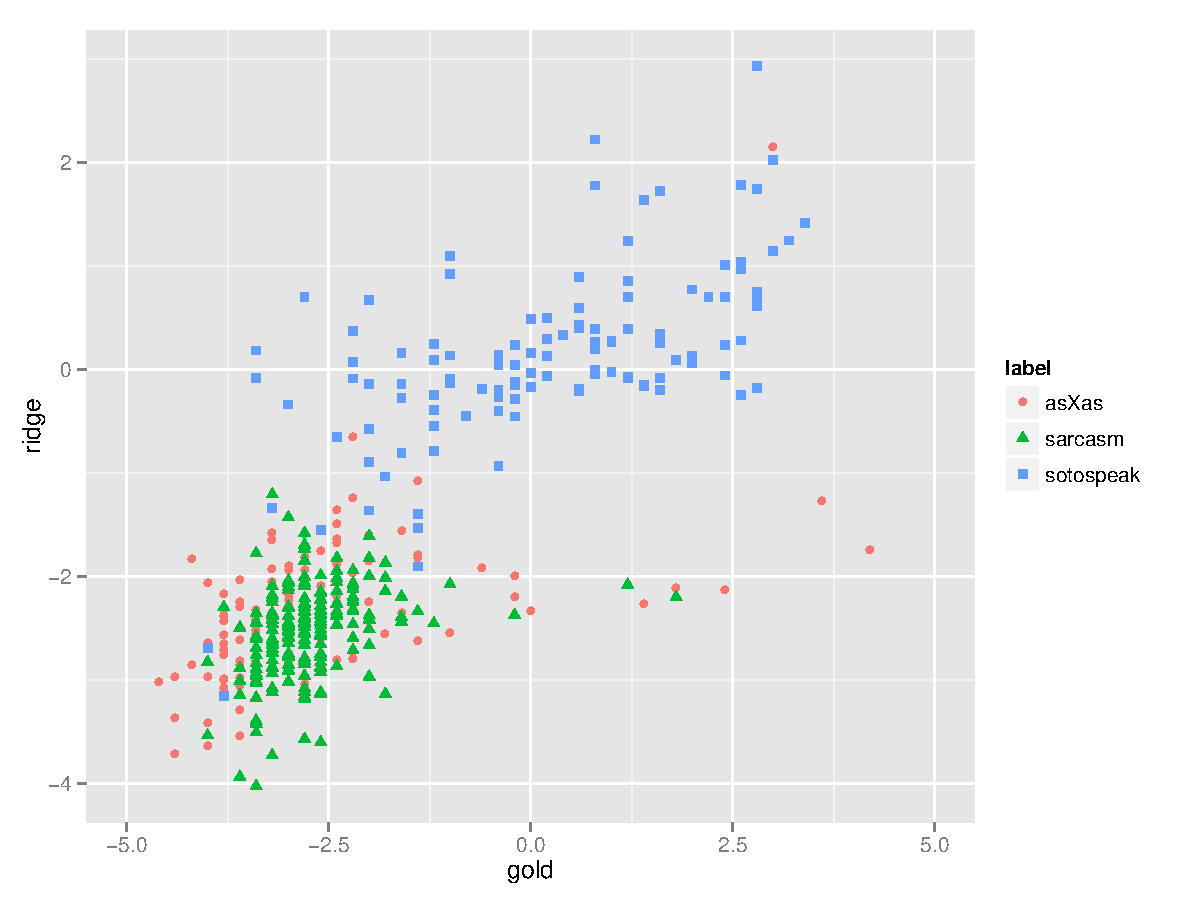
\includegraphics[width=1.05\columnwidth]{trialplotv2.pdf}
    \caption{Label Plots for {\sc RR} predictions.}
    \label{fig:LabelPlot.Sarc.soto.asX}
\end{figure}


\subsection*{The effect of a general sentiment system}
The data for this task is very different from data that most lexicon-based or general sentiment-analysis models fare best on. In fact, running a general sentiment classifier (GSA) described in~\newcite{Elming:ea:2014robust} on the trial data showed that its predictions are actually anti-correlated with the gold standard scores for the Tweets in this task (cosine similarity score of -0.08 and MSE of
18.62). We exploited these anti-correlated results as features for our stacking systems (cf.\ \S~\ref{subsec:Ensembles}). Figure \ref{fig:TrialGoldGSADist} shows the distributions of the gold scores and GSA predictions for the trial data. It shows that the gold distribution is skewed with regards to the number of negative instances to positives, while the GSA predicts more positive sentiment.

\begin{figure}[ht!]
    \centering
    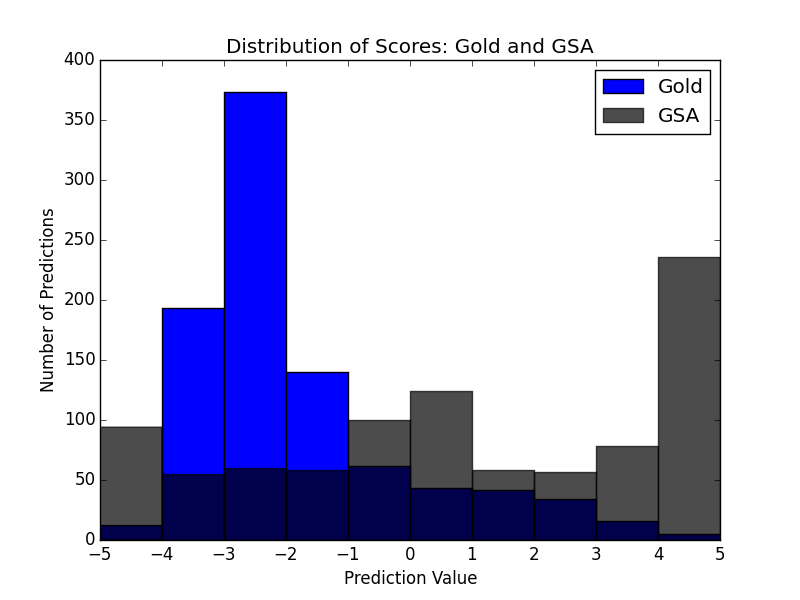
\includegraphics[width=\columnwidth]{gold_gsa_distributions3.png}%{gold_gsa_distributions.png}
    \caption{Distribution of Gold Scores and GSA Predictions for Trial Data.}
    \label{fig:TrialGoldGSADist}
\end{figure}



\section{System Description}
We approached the task~\cite{semevalTask11} as a regression task (cf.\ \S \ref{subsec:forregression}), combined several systems using stacking (\S~\ref{subsec:Ensembles}), and rely on features without POS, lemma or explicit use of lexicons, cf.\ \S~\ref{sec:Features}. %and while not regularly used in NLP it fits well here as the systems predict a real sentiment score in the range [-5.0,5.0].
% We submitted three systems for final evaluation. A ridge regression system which had the best single system performance on the trial data. Further we used two ensemble systems based on stacking. 
%The following gives a brief description of the models, the features are listed in Table~\ref{tbl:featuresTable}.
%The next section describes the models, features are listed in Table~\ref{tbl:featuresTable}.


\subsection{Single Systems}
\label{subsec:SingleSystems}

%\paragraph{Linear Regression (LR)} A linear regression model.
\paragraph{Ridge Regression ({\sc RR})} A standard supervised ridge regression model with default parameters.\footnote{\url{http://scikit-learn.org/}}

\paragraph{PCA\_GMM Ridge Regression ({\sc GMM})} A ridge regression model trained on the output of 
unsupervised induced features, i.e., a Gaussian Mixture Models (GMM) trained on PCA of word n-grams.
PCA was used to reduce the dimensionality to 100, and GMM under the assumption that the data was sampled from different distributions of figurative language, $k$ Gaussians were assumed (here $k$ = 12). 
%The GMM was used under the assumption that the data in the set came from many types of figurative language, and were therefore sampled from different distributions.
%The learning model was ridge regression.
\paragraph{Embeddings with Bayesian Ridge ({\sc EMBD})} A Bayesian Ridge Regressor learner with default parameters trained on only word embeddings. 
A corpus was build from the training data and a Tweet collection sampled with the labels from the TLS and some key words identified from the data e.g. `speak'. 
%The corpus was lowercased and the usernames and URLs in the corpus were normalized to '@USER' and 'URL' respectively. 
This resulted in a total of 3.7 million tweets and 67 million tokens. 
For details on how the word embeddings were built see \S\ref{sec:Features}.



\subsection{Ensembles}\label{subsec:Ensembles}
We developed two stacking systems~\cite{Wolpert:1992}, {\it Stacking System 1} ({\sc St1}) and {\it Stacking System 2: Stacking with Back Off} ({\sc St2}). The systems used for these are shown in Table  \ref{tbl:stackingTable} and the Meta Learner used for both stacking systems is Linear Regression.
%\paragraph{{\sc St2}}

The systems used in {\sc St1} and {\sc St2} are not the only differences between the two. {\sc St2} uses the TLS to identify the subgroup that each tweet belongs to. For any Tweet with the {\sc None} subgrouping, the system would back off to the predictions from the GSA. We built {\sc St2} as a system that is not limited to sentiment analysis for a small subsection of language, the phenomenon of figurative language, but is applicable in situations covering many types of Tweets including those in which literal language is used.

\begin{table}[ht!]
\begin{center}
\begin{tabular}{c || c c}
Single System / Stacking System & {\sc St1} & {\sc St2}\\
\hline
{\sc RR} & X & X\\
{\sc GMM} & X & \\
{\sc EMBD} & &X\\
{\sc GSA} & X&X \\
\end{tabular}
\end{center}
\caption{Systems in Ensemble Setups.}
\label{tbl:stackingTable}
\end{table}

%\section{Features}
\subsection{Features}

\label{sec:Features}

This section describe the features we used for the models in \S \ref{subsec:SingleSystems}. Table \ref{tbl:featuresTable} indicates the type of features used for the single models. Punctuation was kept as its own lexical item and we found removing stopwords and normalizing usernames to '@USER'  increased performance and as such the preprocessing methods are the same across the models. Features were set on the trial data.%, this is why different n-grams and n-gram types are used in the models.
%We ran experiments with and without stopwords, and normalising usernames to a standard name, keeping them as they were or removing them altogether. We found that removing stopwords and normalizing usernames increased performance and as such the preprocessing methods are the same across the models. We removed stopwords and normalized usernames to '@USER'.  

\paragraph{Word N-Grams}
Systems use different n-grams as features. In {\sc RR} counts of 1 and 5 word grams, in GMM binary presence of 1,2, and 3 word grams.

\paragraph{Uppercase Words} Counts of the numbers of word in a Tweet with all uppercase letters.

\paragraph{Punctuation} Contiguous sequences of question, exclamation, and question and exclamation marks.

\paragraph{TLS Label} The subgrouping label from the TLS.

\paragraph{Word Embeddings}
Parameters for word embeddings:\footnote{\url{https://code.google.com/p/word2vec/}} 100 dimensions, 5 minimum occurrences for a type to be included in the model, 5 word context window and 10-example negative sampling. Each tweet was represented by 100 features that represented the average of all the embeddings of the content words in the tweet. %{\bf REFERENCE THE TOOL AND PAPER}
\begin{table}[ht!]\centering

%\resizebox{\columnwidth}{!}{
\begin{tabular}{l || c c c}
Features/Systems & {\sc RR} & GMM  &EMBD \\
\hline
Word N-grams & X & X & \\
Uppercase & X& \\
Punctuations &X  & \\
TLS Label & X &\\
Word Embeddings & & &X\\
\end{tabular}
%}
\caption{Features used in Single Models.}
\label{tbl:featuresTable}
\end{table}

\section{Results}

\subsection{Constant baselines \& Single Systems}\label{sec:baselineResults}
%Five baseline systems were constructed. These were the Mean, Mode, Median, Random and TLS baseline systems. The results of these systems are in Table \ref{tbl:baselines}. TLS takes the mean based on subgroups in the data, and interestingly the performance rose from 0.73 to 0.81 cosine similarity. The best performing single system was the {\sc RR} system.
We implemented the Mean, Mode, Median, Random and TSL (\S\ref{sec::dataanalysis}) baseline systems. TSL is the hardest baseline, and {\sc RR} is the only system that beats it.

\begin{table}[!ht]
\begin{center}
\begin{tabular}{|l|r|r|}
\hline
System & Cosine & MSE\\
\hline
TLS & {\bf 0.81} & {\bf 2.34}\\
Mean & 0.73 & 3.13\\
Mode & 0.73 & 3.13\\
Median & 0.73 & 3.31\\
Random & 0.59  & 5.17\\
\hline
{\sc RR} & {\bf 0.88} & {\bf 1.60}\\
%LR & 0.87 &1.67\\
GMM & 0.79  & 2.55\\
EMB & 0.78 & 2.64\\
\hline
\end{tabular}
\end{center}
\caption{Baseline and Single Systems On Trial Data.}
\label{tbl:baselines}
\end{table}




%\subsection{Single Systems Results}
%Table \ref{tbl:regressionResults}  shows the performance of  the single systems discussed in \S \ref{subsec:SingleSystems}. The best performing single system was the {\sc RR} system.

%\begin{table}[ht!]
%\begin{center}
%\begin{tabular}{|l|r|r|}
%\hline
%System & Cosine & MSE\\
%\hline
%{\sc RR} & 0.88 & 1.60\\
%%LR & 0.87 &1.67\\
%GMM & 0.79  & 2.55\\
%EMB & 0.78 & 2.64\\
%\hline
%\end{tabular}
%\end{center}
%\caption{Regression Model Results.}
%\label{tbl:regressionResults}
%\end{table}

\subsection{Results Stacking Systems}
The performance of the stacking systems on the trial data can be seen below in Table \ref{tbl:stackingResults}. {\sc St2} did not perform well on the trial data although a reason for this is that only 7\% of the trial data was found as not belonging to a known figurative type of tweet.

\begin{table}[ht!]
\begin{center}
%\resizebox{\columnwidth}{!}{
\begin{tabular}{|l|r|r|}
\hline
System & Cosine & MSE\\
\hline
{\sc St1} & 0.86 &1.88\\
{\sc St2} & 0.79 & 2.57\\
\hline
\end{tabular}
\end{center}
%} % end resize box
\caption{Stacking Model Results on Trial Data.}
\label{tbl:stackingResults}
\end{table}
 
\subsection{Final Results} 

Three models were submitted for final evaluation on the test data. The three models were {\sc RR}, {\sc St1}, and {\sc St2}. For the final results we scaled back values outside the range [-5,5] to the nearest whole number in range. 
%This was a requirement of the submissions to avoid penalty for extreme values outside of the range.
%, and the final results were check against gold standard sentiment scores that were integers. 
Tables \ref{tbl:submissionsTest} and \ref{tbl:submissionsCosineBreakdown} show the results for our systems on the final dataset and the performance of the overall winning system for the task ({\sc CLaC}) . Table \ref{tbl:submissionsTest} shows the overall cosine similarity and MSE for the systems on the test data and Table \ref{tbl:submissionsCosineBreakdown} shows the breakdown of the cosine similarity for the systems on the different parts of language. It is interesting to note that the performance of {\sc St2} on the `Other' type of language is identical as the performance for {\sc CLaC}, this is also the best cosine similarity score `Other' out of all submissions.


%The numbers in bold indicate the best performance among our different systems, the `*' indicates the best performance between any of our systems and the winning system.
\begin{table}[ht!]
\begin{center}
\begin{tabular}{| l |  r | r | }
\hline
System  & Test Cosine & Test MSE\\
\hline
{\sc RR}  & 0.625 & 3.079\\
{\sc St1}  & 0.623 &{\bf  3.078}\\
{\sc St2} &  {\bf  0.661} & 3.404 \\
\hline
\hline
{\sc CLaC} & \underline{0.758} & \underline{2.117}\\
\hline
\end{tabular}
\end{center}
\caption{Submission System Test Results.\protect\footnotemark}
\label{tbl:submissionsTest}
\end{table}
\footnotetext{The numbers in bold indicate the best performance among our systems, underlined indicates the best performance between any of our systems and the winning system.}

\begin{table}[ht!]
\resizebox{\columnwidth}{!}{
\begin{tabular}{|l|r|r|r|r|r|}
\hline
System & Overall & Sarcasm & Irony & Metaphor & Other\\
\hline
{\sc RR} & 0.625&0.897&0.886&0.325&0.218\\
{\sc St1} & 0.623&\underline{{\bf 0.900}}& \bf{0.903}&0.308&0.226\\
{\sc St2} & {\bf 0.661} & 0.875 & 0.872 & {\bf 0.453} & \underline{{\bf 0.584}} \\
\hline
\hline
{\sc CLaC} & \underline{0.758} & 0.892 & \underline{0.904} & \underline{0.655} & \underline{0.584}\\
\hline
\end{tabular}
} % end resize box
\caption{Cosine Test Results Breakdown.}
\label{tbl:submissionsCosineBreakdown}
\end{table}

\subsection{The case for regression} 
\label{subsec:forregression}
Regression is less usual in NLP than classification. In this section we show that for this data, it is desirable to use regression. % because it outperforms our best classification model because 
It incorporates the relation between the labels instead of treating them as orthogonal---in addition to the advantage of keeping the decimal precision in the target variable when training.
%We experimented with setting this problem up as a classification problem and tested different models and methods for doing this. 
%Rather than model this task directly as an 11 class problem we used percentiles to bin scores into particular classes and ran experiments to find the best settings. %conversion method from class labels to numeric values, such as assigning the minimum score of all the training instances in that class. 
%We experimented with setting this problem up as a classification task, using percentiles to bin scores into particular classes and ran experiments to find the best settings.
We ran classification experiments for this task but found that the best classification system's\footnote{Decision Tree with 7 classes and using the minimum score for instances in the classes in the training data to convert for class labels to scores.}  %used different conversion methods and the number of classes was always below 11, but its best performance (Cosine 0.82, MSE 2.51) is still far from the {\sc RR} model (0.88,1.60).  
performance (Cosine 0.82, MSE 2.51) is still far from the {\sc RR} model (0.88,1.60). 
%. Table \ref{tbl:classificicationResults} shows the results for the best classification\footnote{Decision Tree with 7 classes and using the minimum score for instances in the classes in the training data to convert class label back to a score. (DT\_7min)}  and regression models.

%\begin{table}[ht!]
%\begin{center}
%\begin{tabular}{| l | r | r |}
%\hline
%System & Cosine & MSE\\
%\hline
%{\sc RR} & 0.88 & 1.60\\
%DT\_7min & 0.82 & 2.51\\
%
%\hline
%\end{tabular}
%\end{center}
%\caption{Classification Model Results on Trial Data.}
%\label{tbl:classificicationResults}
%\end{table}
%

%\section{Analysis}\label{sec:analysis}

%example annotation, example systems\\

%{\em @bumpshow I love these boys so much and I'd be so grateful for the opportunity to speak to them , please \#Bumps5SOSFanCalls <NUM>}



\section{Conclusions}
We tested three systems for their abilities to analyse sentiment on figurative language from Twitter. Our experiments showed that a general SA system trained on literal Twitter language was highly anti-correlated with gold scores for figurative tweets. We found that for certain figurative types, sarcasm and irony, our system's predictions for these phenomena faired well. Our system did not explicitly use a lexicon to define the sentiment of a tweet, but instead used machine learning and strictly corpus-based features (no POS or lemma) to place us 4th in the task. % with a system that could handle both figurative and literal text. 
%We found also that 
%More effort may be needed to determine the type of tweet to focus efforts on the detection of metaphorical and literal tweets to build a more robust system that could better analyse this type of language, although, even for humans the sentiment of tweets is hard to judge as can be seen from the data where a number of tweets were repeated, but did not always share the same gold score.
More effort may be needed to discriminate  metaphorical from literal tweets to build a more robust system, although, even for humans the sentiment of tweets is hard to judge.% This can be seen from the data where a number of tweets were repeated, but did not always share the same gold score.



%\section*{Acknowledgments}

\bibliographystyle{naaclhlt2015}
\bibliography{biblio.bib}
\end{document}
